\documentclass{article}

\usepackage[]{graphicx}
\usepackage[style=apa]{biblatex}
\usepackage[colorlinks=true,citecolor=.,linkcolor=.]{hyperref}
\usepackage[]{microtype}
\usepackage[table]{xcolor}
\usepackage[]{multicol}
\usepackage[toc,page]{appendix}
\usepackage[capitalise]{cleveref}

\addbibresource{final-report.bib}

\begin{document}
\begin{titlepage}
  \begin{center}
    \Large{Raffles Institution \\ Year 2 Research Education \\ Final report} \\
    \vspace{1cm}
    \huge{How to harness green roof technology in schools to encourage
      Singaporean students, through CCAs, to play an active role in reducing
      carbon footprints and controlling the negative effects of greenhouse
      gases?
    } \\
    \vspace{1cm}
    \large{
      \textbf{Authors}: \\
      Nathaniel Chong(3) \\
      Lee Jun Wei(13)\footnote{Group leader} \\
      Teng Zi Huan(28) \\
      Isaac Yeo(32) \\
      \vspace{1cm}
      \begin{tabular}{r@{:}l}
        \textbf{Class} & \hspace{1cm} 2F \\
        \textbf{Teacher} & \hspace{1cm} Dr. Tan Guoxian \\
      \end{tabular}
    }
  \end{center}
\end{titlepage}

\newpage

\begin{abstract}
  \noindent{
    In Singapore, many students do not see the need to protect the
    environment. Thus, this study seeks to investigate the feasibility of
    educating Singapore youth about the environment and encouraging them
    to play an active role in environmental protection through the use of
    green roofs in schools. Surveys were conducted, and most respondents
    were secondary school students. Two interviews were also conducted
    with two interviewees from secondary school to gain insight into
    the matter. After further analysis, it was observed that most did
    not really know about green roofs, but had a positive perception of
    green roofs. They also had moderate environmental awareness. Thus,
    active participation in environmental protection through the use
    of green roofs should be possible with more education about green
    roofs and the severity of climate change, and how to play an active
    role in minimising their carbon footprint.
  }
\end{abstract}

\newpage

\tableofcontents

\newpage

\begin{multicols}{2}

  \section{Introduction}
  \subsection{On green roofs}
  \subsubsection{Definition}
  \paragraph{} Green roofs involve growing plants on roofs, which can
  be sorted into muscinal roofs, herbaceous roofs and arbustive roofs
  \parencite{ecoeng}.


  \subsection{Benefits}
  \subsubsection{Summary}
  \paragraph{} They can reduce energy demand on space conditioning,
  help in purifying air, and if widely adopted, could reduce the urban
  heat island effect, among other benefits \parencite{energeff}.


  \subsubsection{Economic}
  \paragraph{} Research on green roof technologies has so far proven them
  beneficial, with \cite{energeff} mentioning that they can reduce energy
  demand on space conditioning and decrease temperature fluctuations. This
  is agreed on by \cite{CFGRSG} who states that increased roof insulation
  could reduce space conditioning required in the building. Other
  sources also mention the decreased carbon emissions due to lower energy
  consumption from improved thermal performance \parencite{CommAwareGBSyd}
  which reduces cost of energy as there will be up to a 75 percent
  decrease in energy usage for cooling the building, with daily averages
  dropping from 7.5kWh to 1.5kWh \parencite{energeff}. \cite{energeff} also
  mentions that daily temperature fluctuations on roofing membranes are
  significantly reduced, which can increase the lifespan of the roof.


  \subsubsection{Environmental}
  \paragraph{} \cite{energeff} states that if green roof technologies
  are widely adopted, they could reduce the urban heat island effect (a
  situation where an urban area has higher temperatures than surrounding
  rural areas) by having the plants on the green roofs absorb some of the
  heat. \cite{HKGreenRoofGL} also suggests that it “mitigates the urban
  heat island effect”. It is also said that green roofs can increase the
  aesthetics of urban landscape, reduce glare for surrounding buildings,
  showing its importance and relevance in today's highly urbanised
  society. Additionally, \cite{HKGreenRoofGL} found that green roofs
  can mitigate air quality issues, which are important for the wellbeing
  of all. Therefore, we find that there is a need to educate students,
  especially those in secondary institutions (as they are mature enough to
  understand the gravity of global warming and climate change and the need
  to take immediate action, and are more likely to have time to undertake
  this project than those in tertiary institutions) about green roofs.
  Vegetation on green roofs help purify the air and convert carbon
  dioxide into oxygen, which reduces the amount of greenhous gases in
  the air. \parencite{energeff} mentions this, and \cite{CommAwareGBSyd}
  goes a step further, even suggesting that green roofs help achieve zero
  carbon footprints. The plants also take in rainwater, reducing the
  water in the sewage system which needs to be purified and discharged
  to the sea, helping to stabilize the groundwater level and reducing
  the possibility of the sewer clogging and malfunctioning.



  \subsection{Purpose and significance of research question}
  \subsubsection{Purpose}
  \paragraph{} To find ways to, through green rooftop technology, increase
  Singapore students' awareness of climate change and how they can play
  a part in reducing it. See below for more information as to how this
  topic is relevant to today's dynamic and modern society.

  \subsubsection{Significance}
  \paragraph{} Climate change is of significant importance. According to
  \cite{nasa}, at the rate of climate change we are at, the sea levels
  worldwide would increase by 1--4 feet. This leads to the question of
  whether Singapore would truly be safe in the future. This thus draws
  the necessary attention and action of the Singapore Government and the
  citizens. Actions required includes educating the youth of the society
  of the consequences of climate change and the possible course of action.
  However, students in Singapore have ``major gaps in their understanding
  [of climate change]"\parencite{student_carbon_footprint}. Therefore,
  it is necessary for us to research methods that can be used to raise
  awareness of climate change in Singaporean students. At the same
  time, we believe that green roofs can be an effective measure in
  fulfilling its purpose in combating climate change and in motivating
  the Singaporean youth to play an active role in it. Green roofs are a
  potential way to not only encourage the next generation of Singaporeans
  to take climate action,  when the country is in their hands. Proper
  education of the youth would, hopefully, eventually lead to a rise in
  green technology and build a greener, healthier world for everyone
  to live in, one that is possibly freed of the grasps and struggles
  of climate change. Even in Singapore, green roofs have been utilised
  on buildings such as the Nanyang Technological University’s School
  of Art, Design and Media. According to \cite{greenbuild_advant1},
  green roofs not only play a part in helping to slow climate change,
  they also help create a better environment for residents.


  \subsection{Target Audience}
  \paragraph{} We chose secondary school CCAs as our target audience as
  they are old enough and mature enough to understand the implications
  of global warming and climate change, and global warming. They will
  also be the leaders of tomorrow, so it is even more important for them
  to understand this.


  \subsection{Adoption}
  \paragraph{} If adopted in schools by having students to take care
  of and keep up the green roofs, the students would then build this
  habit of caring for and maintaining a green roof, something they would
  hopefully continue to do upon reaching adulthood in the future when
  they would be able to realise human impact on the environment. This is
  even more important should they become national leaders, who have the
  power to influence the lives of other people. Having this influence
  from young, they would then turn to such technologies which can affect
  climate change for the better.

  \section{Methodology}
  \subsection{Purpose}
  \paragraph{} We believe that green roofs are severely underused
  in Singapore despite the advantages, and think that schools are a
  great place to have them implemented. The surveys and interview we
  conducted were in order to find out Singaporean students’ awareness
  and perception of green roofs, as well as the viability of, and their
  willingness to assist in green roof projects in schools.

  \subsection{Interviews}
  \paragraph{} Two interviews were conducted. To have more accurate and
  fair data, we chose two interviewees from two different schools and
  different genders. We carried out the interview on 28 June 3pm. As
  both interviewees were unable to use Microsoft Teams due to a lack
  of access, we used other means to conduct the interview, such as Zoom
  or Discord video calls. The first interviewee was a girl studying in
  Nanyang Girl High, and the second was a boy studying in West Spring
  secondary. This is to ensure diversity and fairness as both parties
  may have certain bias held against green roofs.

  \subsection{Surveys}
  \paragraph{} The survey respondents came from two different age groups:
  primary and secondary school students. In total, we received survey
  responses from 21 students, one of which was not a serious response
  (evident from the options selected, which were all falling in the
  ``Strongly disagree", ``False", or similar categories, even disagreeing
  to the PDPA clause). Hence, we chose to omit the data gathered from
  that respondent and focus on the other 20 respondents. However, 19 of
  the remaining 20 respondents indicated that they were of 13--17 years
  of age, and hence the demographics of our survey were quite limited
  and the data collected may (unfortunately) not be representative of
  the entire student population in Singapore.


  \section{Results}
  \subsection{Summary and results}

  \begin{figure*}
    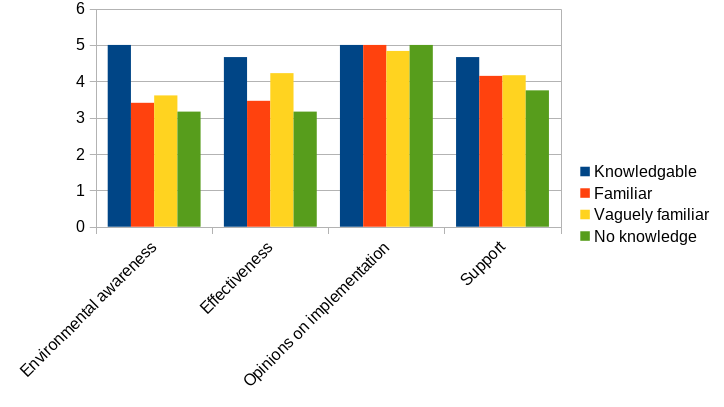
\includegraphics[width=\linewidth]{knowledge-opinions.png}
    \caption{Knowledge of respondents against what they think of green roofs}
    \label{fig:know-opn}
  \end{figure*}

  \paragraph{} In general, we found that the majority of Singaporean
  students are supportive of the concept of green roofs. Furthermore,
  as is shown in \cref{fig:know-opn}, respondents with more knowledge of
  green roofs were, on average, more environmentally aware and showed
  more support, and thought they were more effective in general.


  \subsection{Interpretation}
  \paragraph{} These results showed that in general, teenagers in
  Singapore were supportive of the idea of green roofing. When asked about
  the practical usage of green roofs, 95\% of respondents agreed on all
  aspects that they believed green roof systems being implemented would
  be a good idea. The one respondent that did not agree on every aspect
  noted that building green roofs was a waste of effort, but agreed on
  all other parts. 

  \subsection{Analysis}
  \paragraph{} We noticed that despite the varying levels of understanding
  of green roof systems, there was no clear and specific pattern
  where acceptance and questions regarding the use of green roofs was
  concerned. The questions to gauge their understanding were based on
  two research papers by \cite{HKGreenRoofGL} and \cite{energeff},
  but respondents often showed varying degrees of agreement across
  those aspects listed. This suggests that despite their indication of
  their understanding of green roofs, their actual understanding may
  be different, or due to their individual perceptions. Hence, it was
  difficult to come up with sub group analysis.  Interestingly however, we
  also noticed that when comparing the responses of people who indicated
  that they were only 'vaguely familiar' with green roofs were generally
  more optimistic about than ones who indicated that they were 'familiar'
  with them. Unsurprisingly, though, the single respondent who indicated
  that he was "knowledgable" about green roofs was the most optimistic,
  fully agreeing to most of the statements.



  \section{Social factors regarding green roofs}
  \subsection{General perception of green roofs}
  \paragraph{} \cite{CommAwareGBSyd} found that 55 percent of respondents
  to a survey conducted “strongly agreed” that greenery was important
  and its benefits outweighed its additional costs, showing public support
  of this idea suggesting that our idea may be quite welcome. This is
  supported by \cite{CFGRSG}, who said that with therapeutic value of
  greenery in reducing stress already established, green roofs are used
  commonly in Singapore to soften the harsh urban environment and to
  improve the quality of life. Modern green roofs are now mainly based on
  cost, energy, water savings and carbon reduction \cite{CFGRSG}.  71.8
  percent of respondents in a survey conducted by \cite{CommAwareGBSyd}
  stated that greenery would make a place more attractive to live in
  meaning that greenery could have a positive impact on people’s
  lives, especially for students who spend time in school. However,
  \cite{GRBuildEnSave} also found that 33.8 percent of respondents to
  their survey had less than a general understanding of the concept of
  green roofs--- with the oldest(76+) and youngest(12--17) age groups
  showing the least understanding, further stressing the need to educate
  students about green roofs, although this may be inaccurate due to
  the small sample size. However, \cite{student_carbon_footprint}, also
  found that students in Singapore do not fully understand climate change.



  \section{Discussion}
  \subsection{Possible implementations}
  \paragraph{} We propose that students be grouped according to three
  different CCA groups: sports, performing arts and uniformed groups,
  with each group doing its own part. The students in sports CCAs
  and uniformed groups will carry out the physically more demanding
  tasks (e.g.doing the actual planting itself and taking part in
  maintenance with the assistance of professionals, etc.) since they
  are more used to carrying out such physical tasks than the students in
  performing arts CCAs. The students in performing arts CCAs can manage
  the logistics(planning projects, budgets, etc.) seeing that they are
  likely to be less physically inclined while everyone still keeping to
  the recommended guidelines by \cite{HKGreenRoofGL}.



  \section{Conclusion}
  \paragraph{} Current research has shown that green roofs can be
  beneficial by maintaining a stable temperature, reducing space
  conditioning, amongst other benefits. However, there is still
  a knowledge gap where Singaporean students' perceptions of green
  roofs and its viability in schools are not addressed which is why our
  research is relevant and necessary.

\end{multicols}

\printbibheading
\printbibliography

\newpage

\begin{appendices}
  \section{Research project timeline}
  \begin{table}[h!]
    \begin{center}
      \caption{Our Timeline}
      \label{tab:timeline}
      \begin{tabular}{|c|c|}
        \rowcolor{cyan}
        \textbf{Time} & \textbf{Goal} \\ \hline
        T1W5--T1W9 & Group Project Proposal \\ \hline
        \rowcolor{gray}
        T1W9--T2W3 & Literature review \\ \hline
        T2W3--T2W7 & Finish finalised survey \\ \hline
        \rowcolor{gray}
        T2W7--T3W1 & Administer survey \\ \hline
        T3W1--T3W4 & Data analysis \\ \hline
        \rowcolor{gray}
        T3W3--T3W9 & Prepare for oral assessment \\ \hline
        T3W4--T3W10 & Finalise written report \\ \hline
      \end{tabular}
    \end{center}
  \end{table}
\end{appendices}


\end{document}
